\chapter{Research Methodology}

\section{Research goals}

The goal of this research is to determine whether an adaptive covert communication system is feasible, and if so, to what extent. This will be done by creating a framework for an adaptive covert communication system.
In order to evaluate the framework against the objectives outlined in \fullref{ch:objectives}, a testing environment is required.

\section{The testing environment}
\label{sec:testing_environment}

The requirements of the testing environment are as follows:

\begin{enumerate}
    \item The environment must allow the proposed framework to run.  % 1
    \item The environment must be able to be monitored. % 2
    \item The environment must mimic a real-world network. % 3
    \item The environment must be repeatable. % 4
    \item The environment components must be static. % 5 
    \item The environment must exist on a single machine. % 6
    \item The environment must be controlled, and completely isolated from the non-testing network. % 7
\end{enumerate}


Requirements 1-5 are required to ensure that testing is possible, and that test results are repeatable and comparable. The 6th requirement is a product of my limited resources, and the 7th is due to the limitations of my ethical approval.

These requirements can be met by creating a virtual network, many tools allow for this but in order for the framework to be possible the tool must allow for raw socket access.

Docker \citep{docker} is a tool that allows for the creation of containers inside virtual environments, these containers are lightweight and therefore many can be run on a single machine. this allows for an approach where each function has its container that can be altered as needed. For example, the sender and receiver exist as separate containers, and the traffic generator exists separately from them as well. This makes it easy to restructure and alter the environment as needed.

The shortcomings of Docker however was the lack of ability to capture the traffic of the entire network from inside the environment, it instead had to be done by the host machine. This is not ideal as I'd like to be able to have a completely closed system that can be run in multiple instances to collect data from multiple runs. This would be a useful feature in testing as the covert channels are slow and thus data takes a long time to collect.

Another issue with Docker was the framework didn't work while using it, whereas it did work on my host. Later on in the project, I discovered that the checksum calculations were incorrect, causing the packets to be discarded at the bridge, it is possible that this issue was occurring in Docker, but I had already settled on a different environment at this point.

\subsection{Network namespaces}

Network namespaces are a Linux kernel feature that allows for the creation of virtual network stacks, allowing the simulation of multiple network interfaces. The namespaces came with some other advantages:

\begin{itemize}
    \item The framework runs on bare metal, there is no added overhead of starting a virtual machine.
    \item They exist in the same filesystem as the host, allowing for easy access to the framework source code.
    \item Adding devices and connecting namespaces is easy and scriptable.
\end{itemize}

The structure of the namespaces is as follows:

\begin{figure}[H]
    \centering
    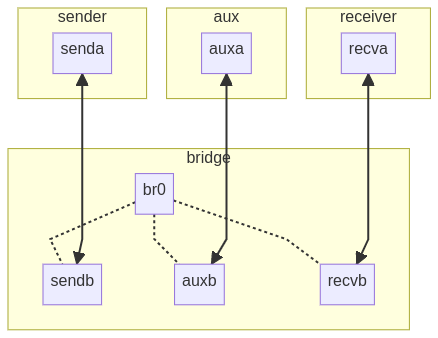
\includegraphics[width=0.5\textwidth]{fig/namespace_setup.png}
    \caption{Diagram of the network namespaces}
    \label{fig:namespace_diagram}
\end{figure}

In the above diagram, the interfaces *a \& *b are virtual ethernet pairs, these are used to connect the namespaces. Only the interfaces that are in their namespace are assigned addresses, the others do not require configuration to work, they are simply used to connect the namespaces.

The reason they are in separate namespaces is to remove ambiguity as to which is the correct interface and route to take, for example, if the sender and receiver were in the same namespace, they would try and route traffic through the loopback interface, which is undesirable behaviour. The use of bridging between the namespaces allows for the traffic to be routed via a central point, which allows for a simple warden to be implemented with access to all the traffic.

A shortcoming of the network namespace is how the traffic moves between namespaces, as a particular namespace can only see traffic that was sent from or to it. This means that the traffic generator must be in the same namespace as the sender, but this is not a problem for a single instance of the framework.

\subsection{Traffic generation}

The traffic generator is responsible for making the environment appear to be a real-world network, for this to also be repeatable the traffic must be generated in a deterministic way. This is done by using tcpdump, a tool that allows packet captures to be replayed via a network interface, allowing a single packet capture to be replayed multiple times.

The next step is then getting a capture of real-world traffic, as per my ethical approval I am not allowed to capture traffic that contains other people's data, so I instead found a public dataset \url{https://www.first.org/conference/2015/program#phands-on-network-forensics} that contains 24 hours of network traffic, that contains no personal information. It should be noted that the dataset is originally intended for use in forensics, but we aren't looking at the contents of the packets so this is not a concern.

There are a few issues with using this pcap, as the network range differs from the one used in the framework, and addresses of the sender and receiver may also have traffic directed at them, which can cause two responses into the network (one from the capture, and one form the read host), to mitigate these issues the traffic is rebased. Rebasing the pcap requires swapping the start of network addresses to the new range, I could have limited this to only the ethernet header but then some traffic, including ARP, would not work properly, so instead I replaced all instances of the old network address with the new one. This could cause some unusual artefacts in the traffic but it is not a concern for this project. The script used to rebase the pcap can be found in \fullref{sec:apdx_rebase_jl}, although this script does as intended, it was an oversight to not factor in checksums and thus all the packets in the pcap have the incorrect checksum, so they are processed through a second script that recalculates the checksums using the python library scapy \cite{scapy}, this script can be found in \fullref{sec:apdx_fix_checksum_py}.

\subsection{Version management}

Both the framework and the testing environment must remain the same for testing to be repeatable, so maintaining version control is important.

\subsubsection{Source control}

To ensure testing is repeatable, the source code that is used must remain the same, and the versions of the dependencies must also remain the same. I achieved using git \citep{git}, a version control system that allows for the tracking of changes to files, and the ability to revert to previous versions. Each commit of changes is uniquely identifiable so it is easy to identify which version of the code was used for a particular test.

Since the testing environment is a superset of the framework, the framework is included as a submodule of the testing environment, this points to a particular commit of the framework, so the framework can be updated independently of the testing environment. This also ensured that commits were atomic and incremental.

For a remote backup of code, I used a private repository on Github \citep{github}, this allowed for the code to be accessed from anywhere, and will allow for the code to be open-sourced in the future.

\subsubsection{Dependency management}

The dependencies of the project are managed by the Julia package manager, it uses a two-file system, one for the dependencies and constraints of the framework \inline{Project.toml} and one that maintains the exact version used \inline{Manifest.toml}. By keeping the \inline{Manifest.toml} file in the repository, the exact versions of the dependencies are known and can be used when the project is cloned, for a repeatable environment.

\subsubsection{External dependencies}

A unique situation arose during the writing of this paper, where a major update was released for Julia, however since I had already begun testing on the previous version, I chose to abstain from updating to the new version. There is not any reason that the code would be incompatible with the new version, but the performance improvements of the newer version would make some of the results incomparable.

The other external dependency used is libpcap \citep{libpcap}, I could include a copy of the library in the repository, but The Tcpdump Group has a good record of compatibility of its library, and then a system specific version can be installed. This is done using the system package manager of choice. 

\subsection{Detecting a covert channel}

I am in a unique situation as the author of this paper, where I know the implementation of the covert channel, and thus detecting the channel is an easier task for me than it would be for an adversary. However, as it is a secure steganographic system \citep{SaW}, my knowledge of the implementation should not allow the detection of the channel with reasonable certainty.

